% In diesem Kapitel soll der Untersuchungsplan zur Bearbeitung der Problemstellung beschrieben werden. Dies beinhaltet Verfahrensweisen und Bearbeitungsschritte, die zur Zielerreichung führen: Was soll auf welchem Weg, wo, wann, in welchen Situationen durch wen ermittelt werden? Es sollte außerdem nachvollziehbar sein, warum bestimmte Methoden verwendet werden und andere nicht (z.B. Abwägung der Vor-/Nachteile in Bezug auf das Thema). Die Komplexität des Untersuchungsplans beeinflusst den Umfang der Arbeit. Bei der Durchführung einer experimentellen Studie, sollte die Grundgesamtheit der untersuchten Fälle oder Personen in allen relevanten Merkmalen so detailliert wie nötig beschrieben werden. Dies gilt in besonderem Maße für die verwendete Stichprobe (bzw. Teilmenge der Grundgesamtheit), weil sie über die Aussagefähigkeit der Untersuchung entscheidet. Ebenso sollte begründet werden, warum die gezogene Stichprobe angemessen
% ist. Wissenschaftliche Kriterien:
% • Die verwendeten Methoden sind unter Vorgabe einer möglichst hohen Qualität hinsichtlich Objektivität, Reliabilität und Validität auszuwählen.
% • Die Durchführung der Untersuchung umfasst die methodisch-organisatorischen Details der Datenerhebung. Diese Beschreibung muss anderen Forschern ermöglichen, die Untersuchung zu wiederholen.
% • Die Auswertungsverfahren sind nur dann ausführlicher darzustellen, falls sie nicht allgemein üblich und bekannt sind (z. B. Eigenentwicklung eines statistischen Verfahren).
% • Forschungsethische Implikationen der Untersuchung müssen bedacht und eventuelle Aushandlungen durchgeführt werden: Wem nützt/schadet die Untersuchung? Welche Rechte haben untersuchte Personen/MitarbeiterInnen?
\chapter{Methodik}
	\section{Funktionsgliederung/-Struktur}
		% Um das Gerät strukturiert konstruieren zu können, werden die einzelnen Funktionen, welche der Arm erfüllen soll, gegliedert.
		Zum Zwecke der Reduktion des Komplexitätsgrades des Gesamtsystems wird sich für das Erstellen eines Funktionsbaumes entschieden. Diese Methode wird bewusst gewählt, um eine einfache Nachvollziehbarkeit und Lesbarkeit zu leisten.\\
		Hier werden die in \cref{chap:Aufgabenstellung} formulierten Anforderungen in grober Form vorstrukturiert, um sich einen Überblick über die Anzahl und Gestalt funktionaler Teilprobleme, sowie möglicher Lösungsansätze zu verschaffen.\\
		Hieraus können in einer frühen Konzeptionsphase bereits unpraktikable Lösungsansätze verworfen und in der textlichen Ausformulierung gegebenenfalls verborgen gebliebene Teilprobleme identifiziert werden.
		Im direkten Anschluss können Kernfunktionen und/oder Lösungsansätze im Rahmen morphologischer Kästen weiter diskutiert werden.	Wie feingliedrig dies geschehen soll, liegt im Ermessen der Konstrukteure.

		\subsection{Funktionsbaum}
			Zunächst werden die allgemeinen Funktionen der Übersicht halber in Kategorien unterteilt. Diese sind in einem Funktionsbaum (siehe \cref{fig:funktionsbaum}) zu sehen.
			
			\begin{figure}[h]
				\centering
				\includesvg[height=.75\textheight]{Abb/chart}
				\caption[Funktionsbaum]{Funktionsbaum.}\label{fig:funktionsbaum}
			\end{figure}

		\subsection{Morphologische Kästen}
			In diesem Unterkapitel wird zur Darstellung von Lösungsmöglichkeiten für Teilprobleme die Methode der morphologischen Kästen gewählt. Diese Methode bringt die Vorteile mit sich, alle Teilprobleme auf einem Blick vor sich liegen zu haben, deren Lösungsoptionen in kompakter Darstellungsweise präsentieren zu können und eine Übersicht anhand Markierung der gewählten Lösungen, welche später teilweise miteinander verknüpft sind und aufeinander beruhen, bieten zu können.\par\medskip
			Zunächst werden aus dem Funktionsbaum kritische Probleme abgeleitet und als Teilprobleme in morphologischen Kästen (s. \crefrange{tab:morphologische-kasten-teilprobleme}{tab:morphologische-kasten-feedback-system}) dargestellt. Da einige Bauteile viele Teilprobleme aufweisen, werden diese in eigenen morphologischen Kästen behandelt.\par
			Im Anschluss werden zu den entsprechenden Problemen Lösungen gesucht und diese dargestellt. Die Lösungen beruhen auf dem Wissen und der Erfahrung des Konstruktionsteams. Die Lösungen werden danach im Hinblick auf verschiedene Kriterien überprüft und die passendste Lösung gewählt. Entscheidende Kriterien dabei sind die Komplexität, die Herstellbarkeit sowie die Kosten.\par\medskip
			In \cref{tab:morphologische-kasten-teilprobleme} werden als allererstes die Teilprobleme aufgelistet, wobei die Baugruppen Schulter, Ellbogen und Handgelenk in \cref{tab:morphologische-kasten-schulter}, \cref{tab:morphologische-kasten-ellbogen} und \cref{tab:morphologische-kasten-handgelenk} eigene morphologische Kästen bekommen, da sie noch einige Unterfunktionen enthalten, für die auch mehrere Lösungsmöglichkeiten infrage kommen. Dasselbige gilt auch für die Teilprobleme des Feedback-Systems in \cref{tab:morphologische-kasten-feedback-system}.

			\begin{table}[h]
				\centering
				\caption[Morphologischer Kasten der Teilprobleme]{Morphologischer Kasten der Teilprobleme.}
				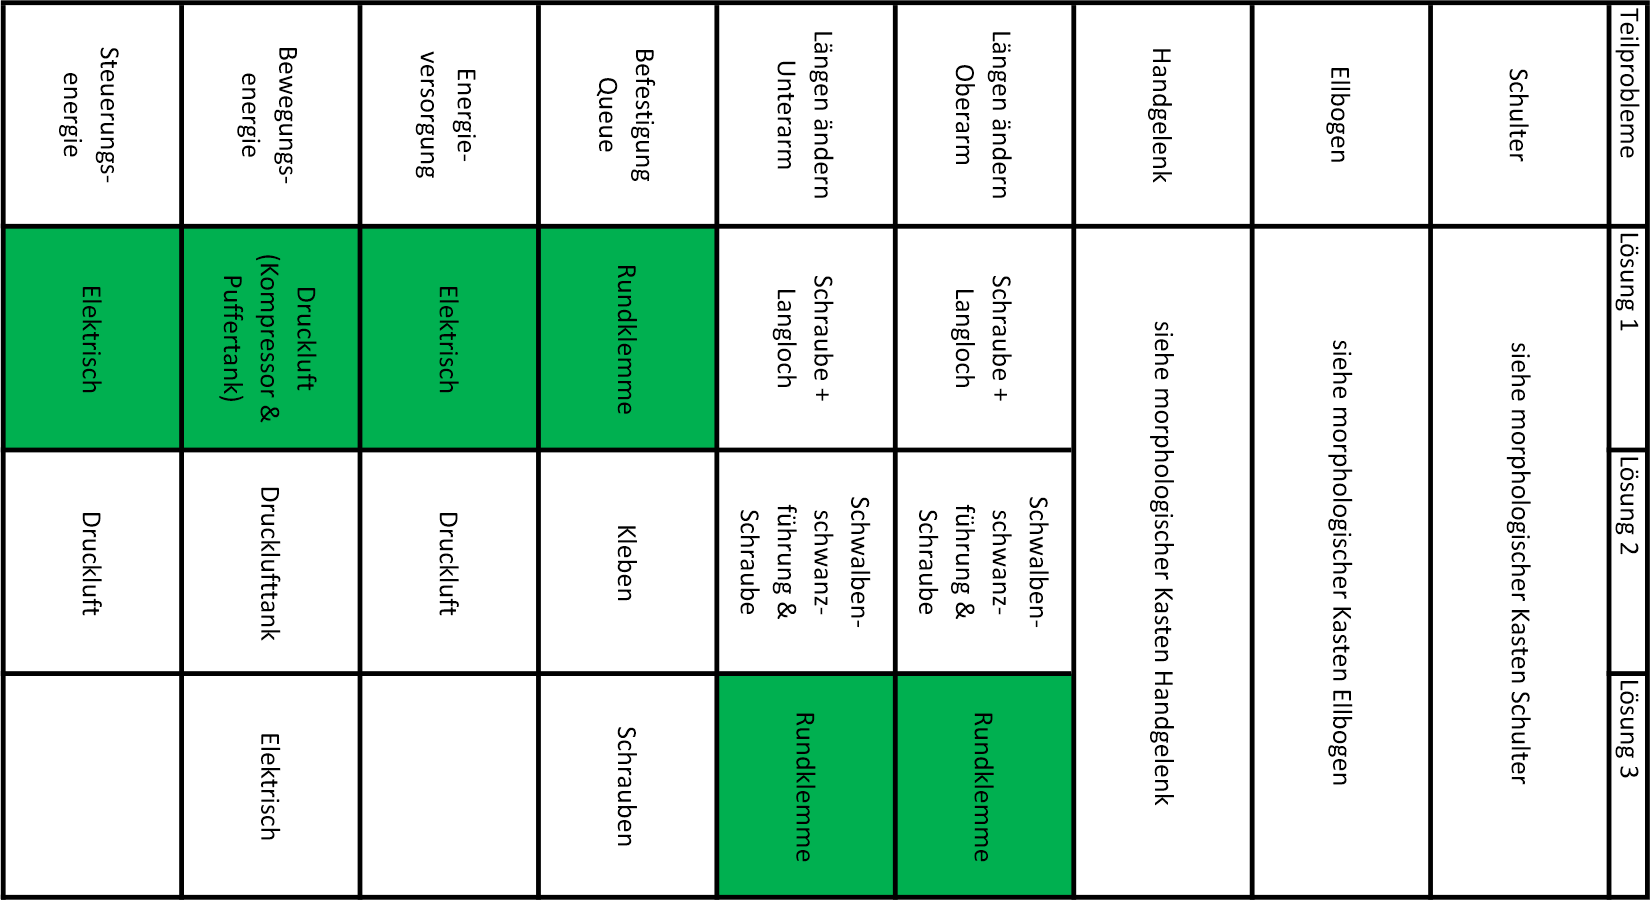
\includegraphics[angle=90, width=.8\textwidth]{Abb/MorphoBoxes/Morphologischer_Kasten_Teilprobleme.png}\label{tab:morphologische-kasten-teilprobleme}
			\end{table}
%
			\begin{table}[h]
				\centering
				\caption[Morphologischer Kasten der Schulter]{Morphologischer Kasten der Schulter.}
				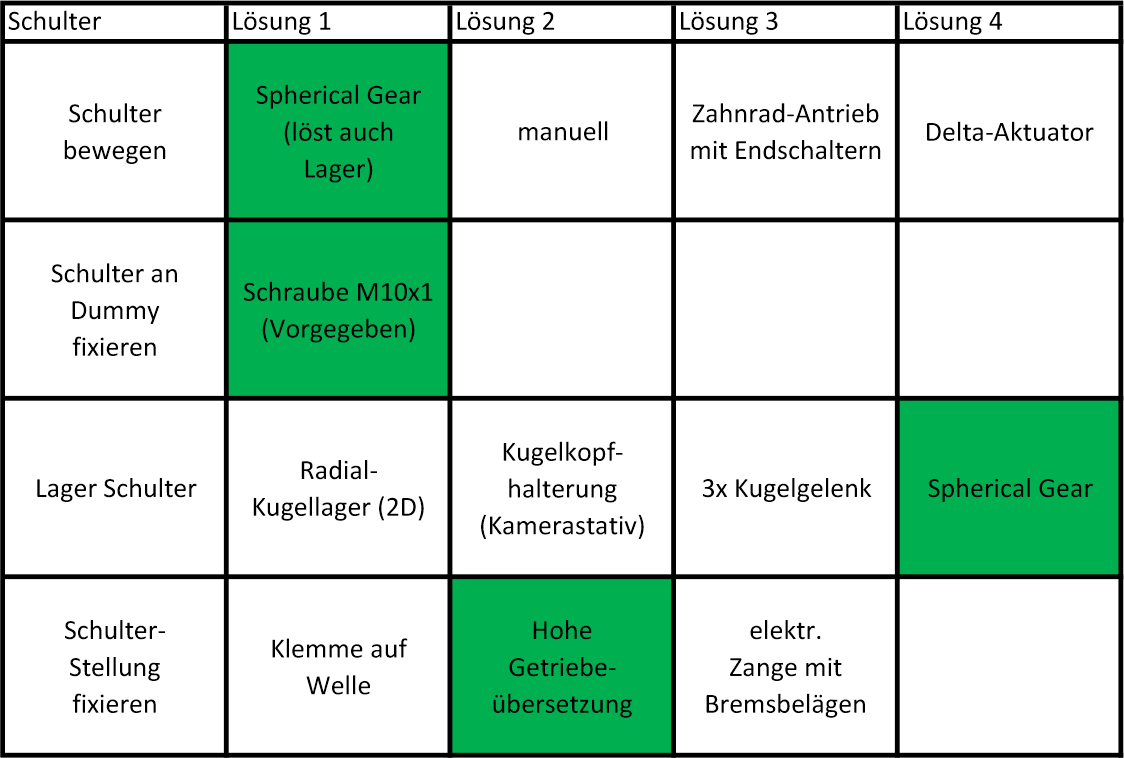
\includegraphics[width=.8\textwidth]{Abb/MorphoBoxes/Morphologischer_Kasten_Schulter.png}\label{tab:morphologische-kasten-schulter}
			\end{table}
%
			\begin{table}[h]
				\centering
				\caption[Morphologischer Kasten des Ellbogens]{Morphologischer Kasten des Ellbogens.}
				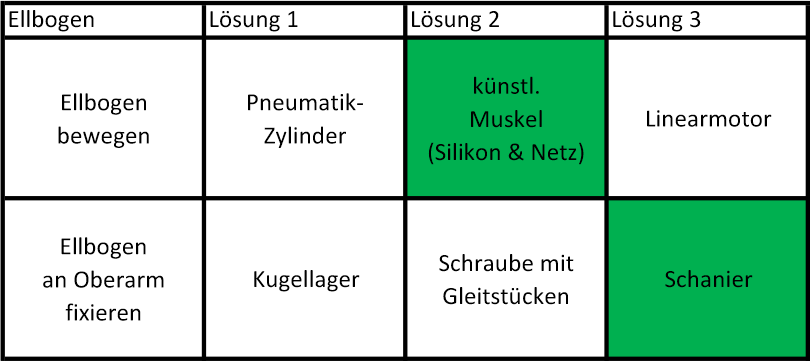
\includegraphics[width=.8\textwidth]{Abb/MorphoBoxes/Morphologischer_Kasten_Ellbogen.png}\label{tab:morphologische-kasten-ellbogen}
			\end{table}
%
			\begin{table}[h]
				\centering
				\caption[Morphologischer Kasten des Handgelenks]{Morphologischer Kasten des Handgelenks.}
				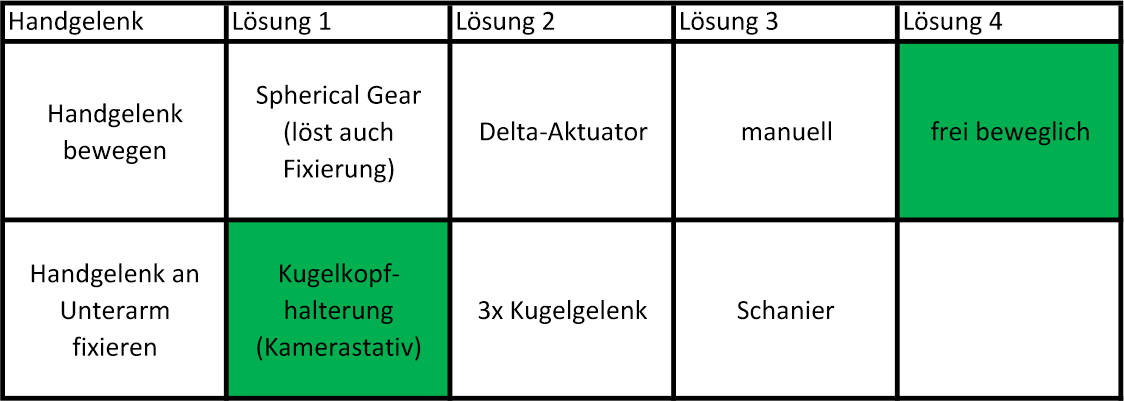
\includegraphics[width=.8\textwidth]{Abb/MorphoBoxes/Morphologischer_Kasten_Handgelenk.png}\label{tab:morphologische-kasten-handgelenk}
			\end{table}
%
			\begin{table}[h]
				\centering
				\caption[Morphologischer Kasten des Feedback-Systems]{Morphologischer Kasten des Feedback-Systems.}
				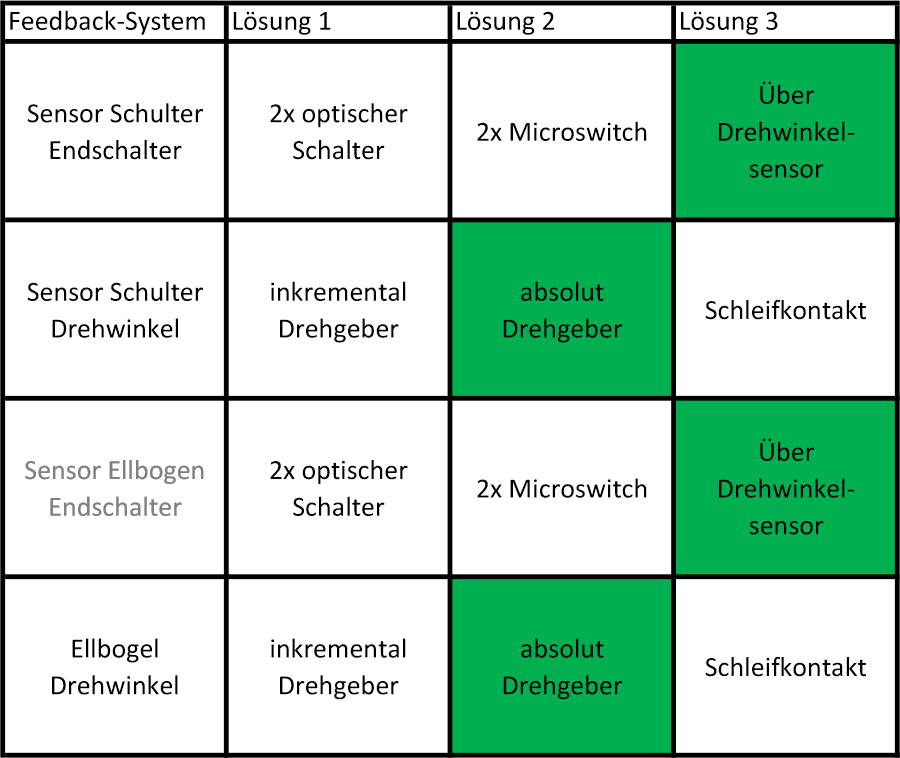
\includegraphics[width=.8\textwidth]{Abb/MorphoBoxes/Morphologischer_Kasten_Feedback-System.png}\label{tab:morphologische-kasten-feedback-system}
			\end{table}

		\subsection{Prinzipskizze}
			Da die Funktionen nun definiert sind, kann das Prinzip des Gerätes schematisch in einer Prinzipskizze aufgezeigt werden.\\
			Sie dient dazu, zu konstruierende Zusammenhänge zu verdeutlichen und bietet eine erste grobe Vorstellung des Geräts. Die bildliche Darstellung hilft außerdem die gewählten Lösungen aus den morphologischen Kästen im vorangegangenen Abschnitt zu verstehen.\\
			\Cref{fig:prinzipskizze-gesamtansicht} zeigt die Hauptbauteile, \cref{fig:prinzipskizze-ellbogen} den Anschluss zwischen Ober- und Unterarm und \cref{fig:prinzipskizze-handgelenk-und-hand} die Hand und ihre Verbindung zum Unterarm.

			\begin{figure}[h]
				\centering
				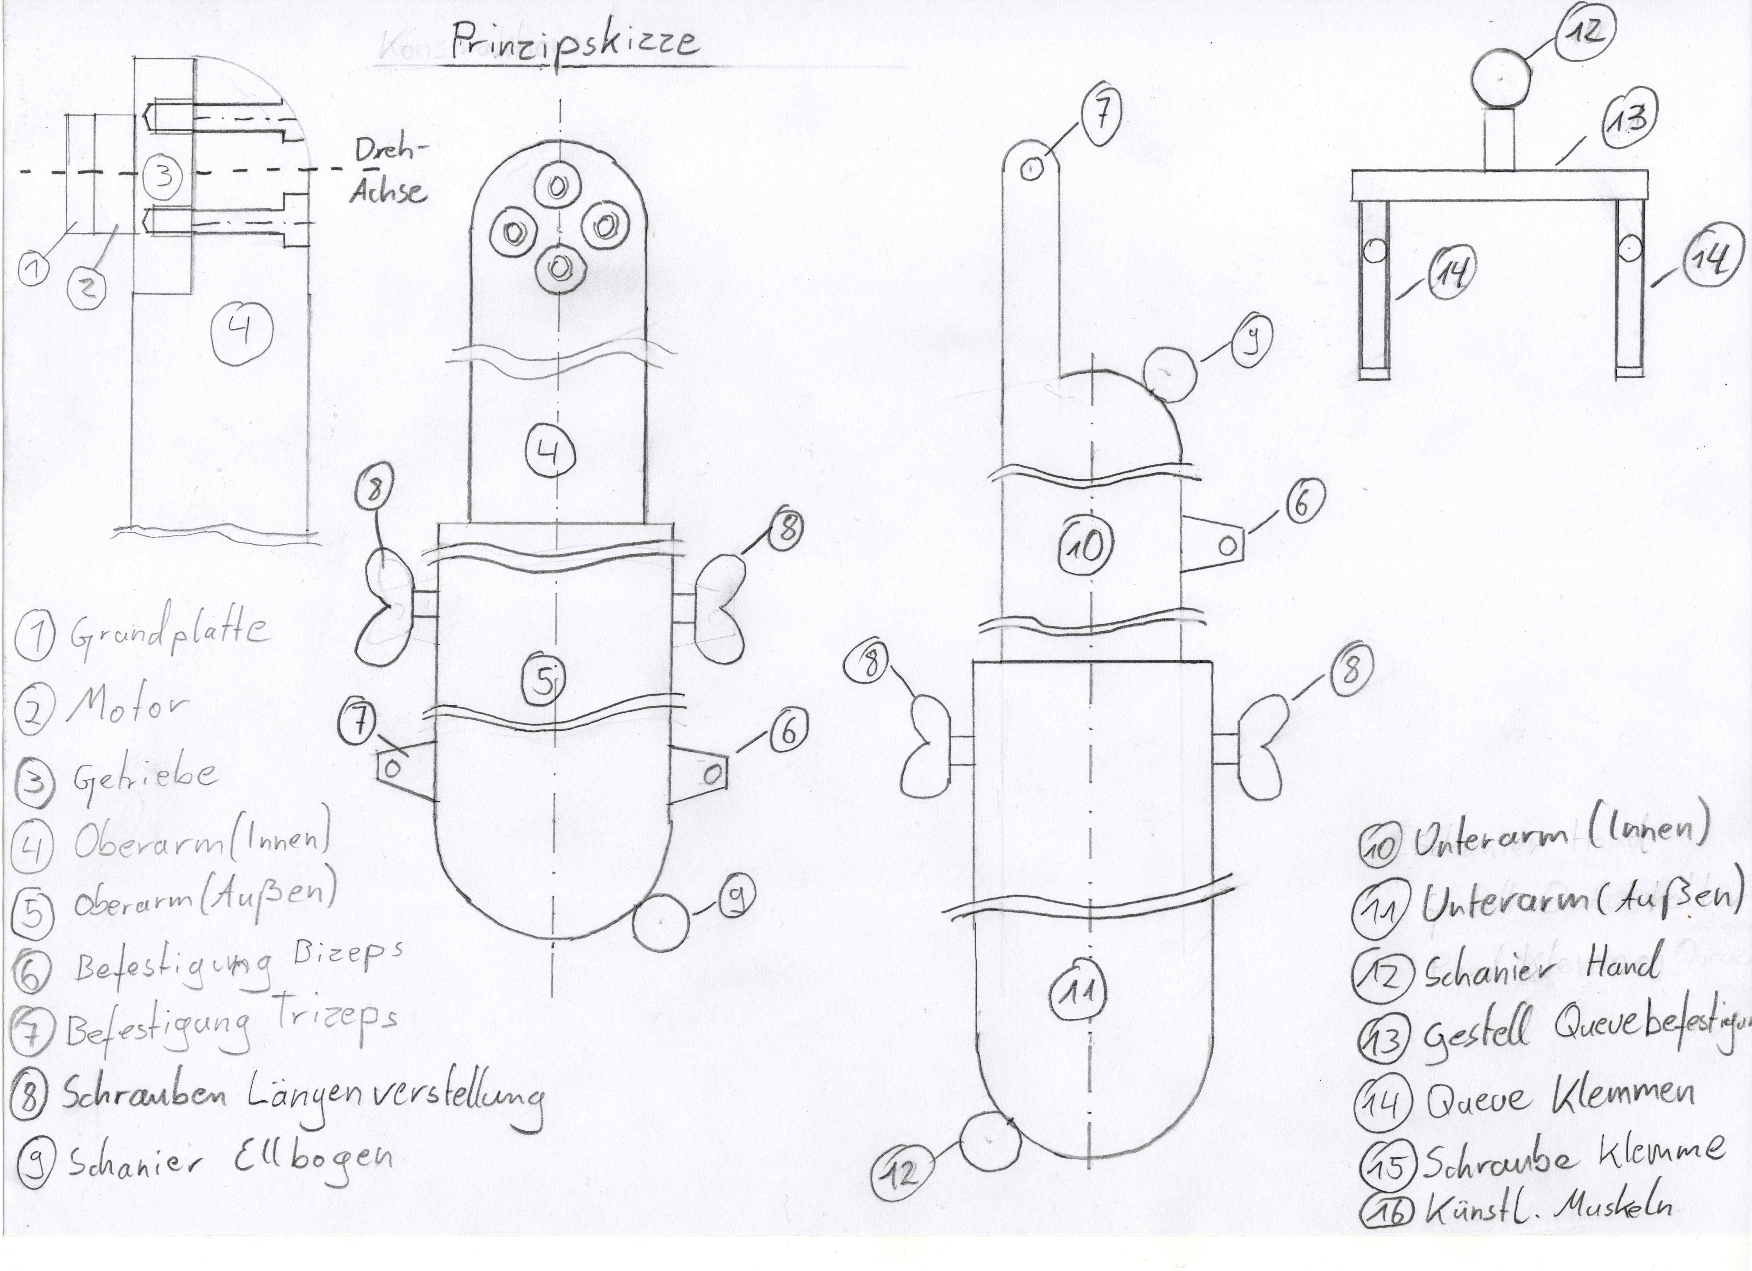
\includegraphics[width=\textwidth]{Abb/Prinzipskizze_Gesamtansicht}
				\caption[Prinzipskizze -- Gesamtansicht]{Prinzipskizze -- Gesamtansicht.}\label{fig:prinzipskizze-gesamtansicht}
			\end{figure}

			\begin{figure}[h]
				\centering
				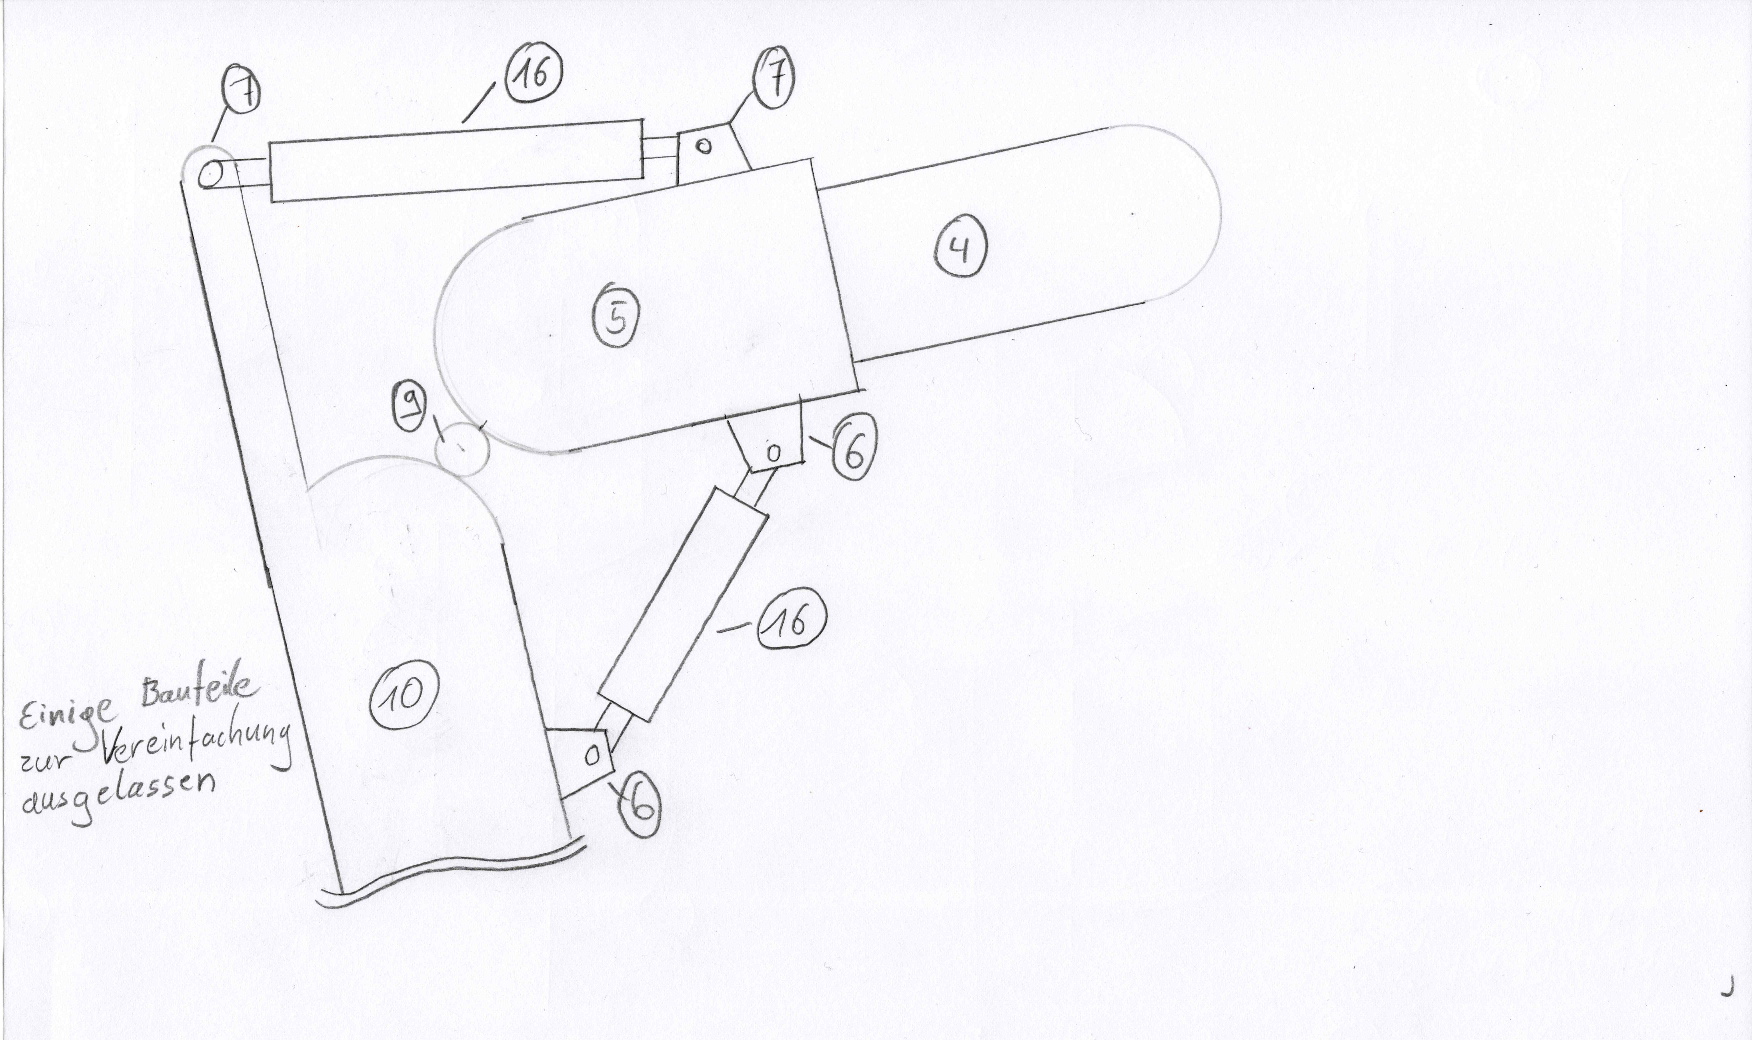
\includegraphics[width=\textwidth]{Abb/Prinzipskizze_Ellbogen}
				\caption[Prinzipskizze -- Ellbogen]{Prinzipskizze -- Ellbogen.}\label{fig:prinzipskizze-ellbogen}
			\end{figure}

			\begin{figure}[h]
				\centering
				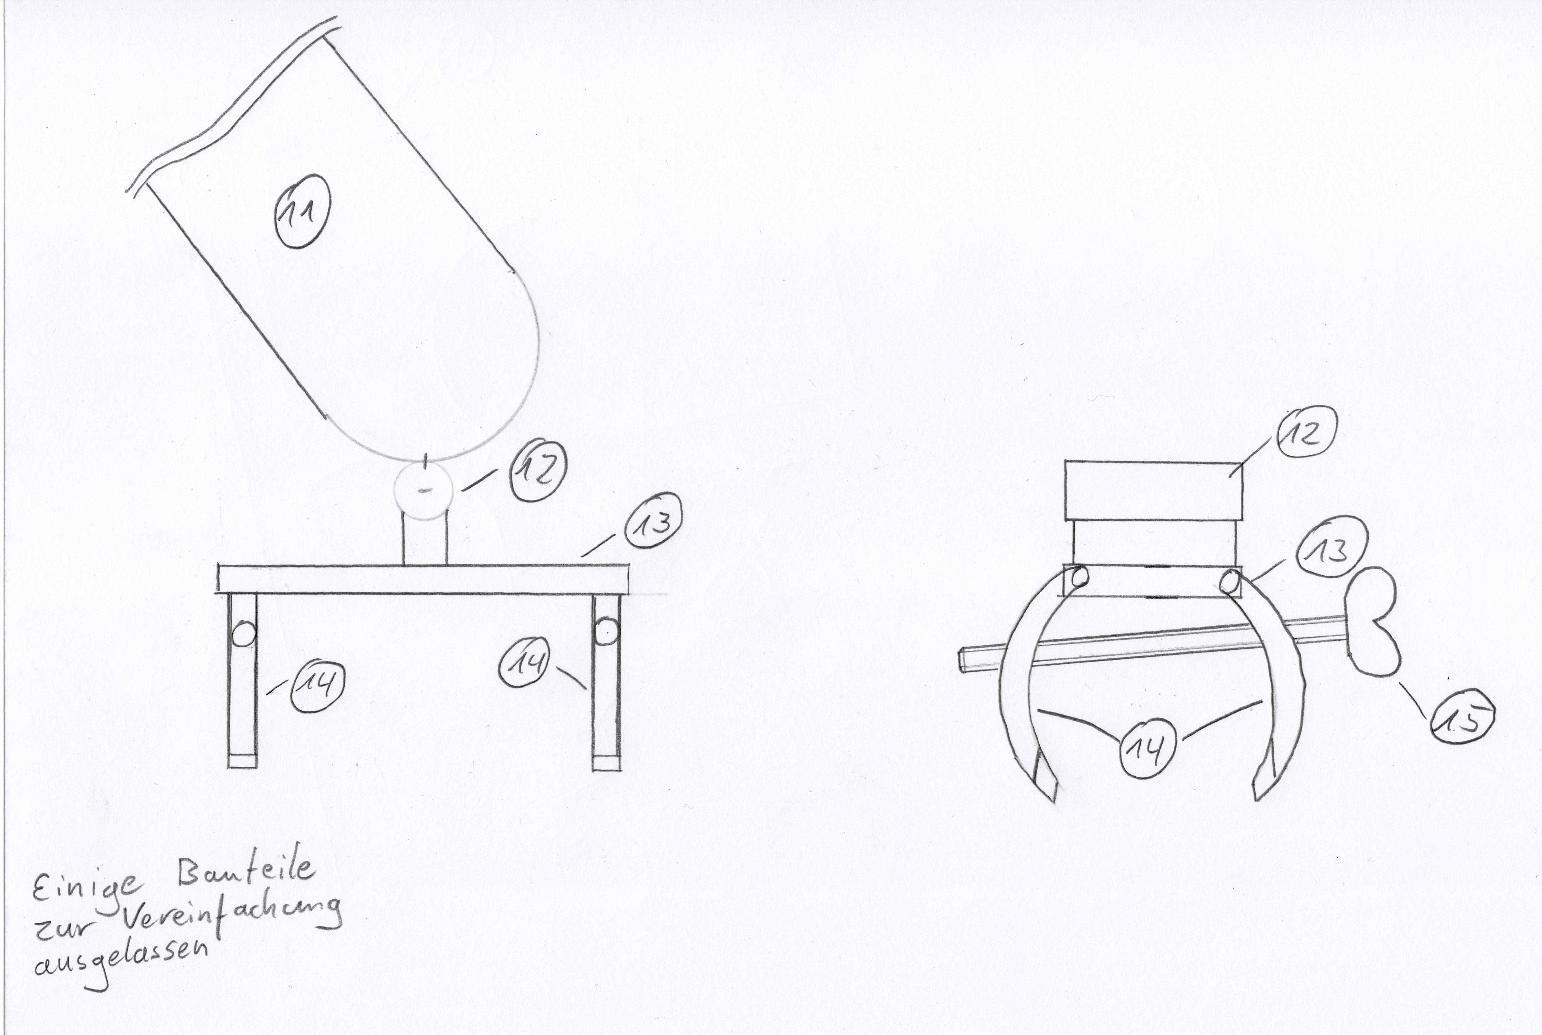
\includegraphics[width=\textwidth]{Abb/Prinzipskizze_Handgelenk_und_Hand}
				\caption[Prinzipskizze -- Handgelenk und Hand]{Prinzipskizze -- Handgelenk und Hand.}\label{fig:prinzipskizze-handgelenk-und-hand}
			\end{figure}

	\section{Begründung der Lösungsauswahl}\label{Begruendung Loesungsauswahl}

		Nun soll erläutert und erklärt werden, wieso die jeweiligen Lösungen aus den morphologischen Kästen ausgewählt wurden.\par\medskip

		Zunächst betrachten wir die übergeordneten Teilprobleme. Dazu zählt unter anderem die Einstellbarkeit der Armlängen. Diese sollen möglichst genau die Anatomie unterschiedlicher Menschen nachbilden. Um dies zu gewährleisten, müssen sie in der Länge verstellt werden können. Die passendste Lösung stellte dabei eine gewöhnliche Fahrradrohrklemme dar. Denn dazu muss nicht zusätzlicher Konstruktionsaufwand betrieben werden, sondern sie können zugekauft werden. Des Weiteren ist an dem Bauteil des Arms wenig Bearbeitungsaufwand. Diese bestehen aus Rohren und können einfach eingeschlitzt werden, um die Verklemmung der Fahrradklemmen auf das innen liegende Rohr zu übertragen. Die Auswahl für die Anpassungsmöglichkeit der Längen ist beim Oberarm und Unterarm identisch.\par\medskip

		Der nächste wichtige Punkt stellt die Befestigung des Queues dar. Dabei muss die Bewegung des Arms auf den Queue übertragen werden. Allerdings darf er sich nicht drehen, da es zu einer ungewollten Bewegung der Kugel führen könnte. Um dies zu gewährleisten, wurde eine Rundklemme gewählt. Sie umschließt den Queue am Griff und ist auch käuflich zu erwerben. Des Weiteren ist sie, anders als die anderen Möglichkeiten, nicht destruktiv.\par\medskip
		
		Die Energieversorgung des gesamten Aufbaus erfolgt mittels elektrischer Energie. Diese ist am einfachsten in andere Energien umzuwandeln und eigentlich überall verfügbar.\par\medskip
		Die Bewegungsenergie bzw. die Energie, die für den Stoß verwendet wird, wird über Druckluft bereitgestellt. Dabei wird sie mit einem mobilen Kompressor erzeugt und in einem Pufferspeicher zwischengespeichert. Sobald der Stoß ausgeführt werden soll, kann die gespeicherte Druckluft kontrolliert abgelassen werden. Bei der Lösung mit nur einem Drucklufttank ist der Nachteil, dass nur so lange Stöße ausgeführt werden können, solange genug Druckluft vorhanden ist. Ist der Tank einmal leer, muss er über einen Druckluftkompressor, die in Billardhallen üblicherweise nicht vorhanden sind, aufgefüllt werden.\par\medskip
		
		Die Steuerungsenergie wird ebenfalls als elektrische Energie bereitgestellt, da damit die Möglichkeit der Ansteuerung von Motoren, sowie das Feedback von Sensoren ermöglicht wird. Eine Steuerung über Pneumatik wäre ebenfalls möglich, allerdings bietet sie nicht die oben genannten Vorteile (vgl. \cref{tab:morphologische-kasten-teilprobleme}).\par\medskip
		
		Wie weiter oben schon erwähnt, wurden einige Bereiche in eigenen morphologischen Kästen aufgearbeitet. Darunter die Schulter, der Ellbogen und das Handgelenk. Diese werden im Folgenden vorgestellt.\par\medskip

		Das erste Teilproblem der Schulter stellte die Befestigung dieser und damit der gesamten Baugruppe an dem bereitgestellten Dummy dar. Allerdings ist der einzige Kontaktpunkt des Dummys eine Schraube mit dem Gewinde M10 $\times$ 1. Diese Lösung ist also von den Gegebenheiten vorgegeben.\par\medskip

		Um einen typischen Billardstoß nachbilden zu können, muss sich außerdem die Schulter bewegen können, da der Arm eines Billardspielers meistens einen Winkel von \SI{90}{\degree} gegenüber der Senkrechten bildet. Da dieser Winkel jedoch von Spieler zu Spieler unterschiedlich ist, musste die Schulter beweglich ausgeführt werden. Um die Bewegung der Schulter umzusetzen, wurde ein spherical gear gewählt, da dies neben der eigentlichen Bewegung auch die Lagerung der Schulter als auch die Fixierung, während eines Stoßes sicherstellt, indem die Getriebeübersetzung entsprechend hoch gewählt wird. Da mit dieser Lösung mehrere Probleme auf einmal gelöst werden können und sie einen relativ kleinen Bauraum einnimmt, wurde diese Variante ausgewählt. Dabei wird allerdings die Bewegung der Schulter auf eine 2D-Ebene beschränkt, was aber für die Nachbildung eines Arms beim Billardspielen keinen Nachteil mit sich bringt (vgl. \cref{tab:morphologische-kasten-schulter}).\par\medskip

		Außerdem muss eine Bewegung am Ellbogen erzeugt werden, da damit die meisten Billardspieler ihren Stoß ausführen. Dabei gab es zwei Probleme zu lösen: Zum einen die Bewegung und zum anderen die Befestigung des Unterarms am Oberarm. Zur Bewegung des Unterarms wurden künstliche Muskeln gewählt. Sie sind flexibel und bilden die menschliche Anatomie sehr genau nach. Um die Bewegung des Arms zu ermöglichen, wurde ein gewöhnliches Scharnier gewählt, da auch dies den Konstruktionsaufwand gering hält und hinzugekauft werden kann (vgl. \cref{tab:morphologische-kasten-ellbogen}).\par\medskip

		Als letztes Problem wird das Handgelenk betrachtet. Dieses muss sich einerseits bewegen und andererseits am Unterarm befestigt werden. Da vom Handgelenk aber bei einer Lagerung des Queues keine eigene Bewegung erforderlich ist wurde die Hand so aufgelegt, dass sie nicht maschinell bewegt werden kann. Als Fixierung und Lagerung wurde am Handgelenk ein 3D-Kugelkopf gewählt, da damit eine genauere Positionierung des Queues möglich ist. So kann er auch in einem Winkel zum Arm ausgerichtet werden und bietet mehr Flexibilität bei der Nachstellung von Stößen (vgl. \cref{tab:morphologische-kasten-handgelenk}).
	\section{Auslegung der Schulter}\label{sec:auslegung}

		\begin{figure}[h]
			\centering
			\includesvg[inkscapelatex=true, width=.6\textwidth]{Abb/schulterauslegung}
			\caption[Vereinfachtes Modell des Systems Schulter-Oberarm-Unterarm]{Vereinfachtes Modell des Systems Schulter-Oberarm-Unterarm mit den Massen \(m_o, m_u\), den Längen \(l_o, l_u\) und dem verursachten Drehmoment \(M_m\).}%
			\label{fig:modell schulter oberarm unterarm}
		\end{figure}
		
		Nach \cite{Soll.1982} entfallen anteilig des Gesamtkörpergewichtes etwa \SI{3}{\percent} auf den Oberarm und \SI{2}{\percent} auf den Unterarm.
		Mit einem angenommenen Gesamtkörpergewicht von \SI{80}{\kilo\gram} entspricht das einem Massenanteil von \SI{2,4}{\kilo\gram} auf den Oberarm und \SI{1,6}{\kilo\gram} auf den Unterarm.
		Hier soll von einer homogenen Massenverteilung ausgegangen werden, womit die jeweiligen Massenschwerpunkte mittig auf der Verbindungslinie zwischen den Gelenken liegt.
		Weiter wird von jeweiligen Längen für Ober- und Unterarm von \SI{0,35}{\metre} und einer Masse \(m_q\) am Ende des Unterarms von \SI{0,5}{\kilo\gram} ausgegangen.\par
		Soll beim Stoß der Oberarm horizontal und der Unterarm orthogonal nach unten gerichtet sein, so befindet sich das Gesamtgewicht des Systems mit \SI{4}{\kilo\gram} entlang der Oberarmachse nach \cref{eq:massenschwerpunkt arme} bei \SI{0,257}{\metre}.

		\begin{align}
			x_s &= \frac{\frac{1}{2}l_o \cdot m_o + l_o \cdot \left(m_u + m_q\right)}{m_o + m_u + m_q} \nonumber \\
				&= \frac{\SI{0,175}{\metre} \cdot \SI{2,4}{\kilo\gram} + \SI{0,35}{\metre} \cdot \left(\SI{1,6}{\kilo\gram} + \SI{0,5}{\kilo\gram}\right)}{\SI{4,5}{\kilo\gram}} \nonumber \\
				&\approx \SI{0,257}{\metre}%
				\label{eq:massenschwerpunkt arme}
		\end{align}

		Um eine stabile Orientierung des Oberarms um das Schultergelenk gewährleisten zu können muss so ein Drehmoment von mindestens \(M_m = x_s \cdot \left(m_o + m_u + m_q\right) = \SI{1,157}{\newton\metre}\) erzeugt werden können.
		Vergleich mit den Kenndaten eines Schrittmotors der Baugröße Nema 23 \cite{nanotec.specs} kann hier im Vollschrittbetrieb ein Haltemoment von \SI{2,95}{\newton\metre} erwartet werden.\par\medskip
		Die genannten Winkelauflösung des Schrittmotors von \SI{1,8}{\degree} übersetzt sich an der Position der Hand zu einer Mindestbogenlänge von
		\begin{align}
			\Delta s_{arc} 	&= \frac{\SI{1,8}{\degree}}{\SI{180}{\degree}} \cdot \pi \cdot l_{eff} = \frac{\SI{1,8}{\degree}}{\SI{180}{\degree}} \cdot \pi \cdot \sqrt{2 \cdot \left(\SI{0,35}{\metre}\right)^2} \nonumber \\
							&= \SI{1,56}{\cm}
		\end{align}
		Hier sei \(l_{eff}\), wie in \cref{fig:schultergelenk winkelaufloesung} dargestellt, die Hypotenuse des durch Ober- und Unterarm aufgespannten Dreieckes.\par
		Da mit nicht-idealen Steifigkeiten der Teilsysteme zu rechnen ist und um Abweichungen durch dynamisches Verhalten im Betrieb auffangen zu können wird eine Untersetzung von \(N = 30\) gewählt.
		Die verfahrbare Mindestbahnlänge \(\Delta s_{arc}\) skaliert umgekehrt proportional mit dem Untersetzungsverhältnis \(N\) aus \cref{eq:untersetzung} gemäß
		\begin{equation}
			\Delta s_{arc} = \frac{1}{N} \cdot \frac{\SI{1,8}{\degree}}{\SI{180}{\degree}} \cdot \pi \cdot l_{eff}
		\end{equation}
		und ergibt sich so für den Fall das gilt \(l_o \perp l_u\) zu \SI{0,5}{\mm}.
		\begin{figure}[h]
			\centering
			\includesvg[inkscapelatex=true, width=.6\textwidth]{Abb/schulterauslegung-winkelaufloesung}
			\caption[Die effektive Länge \(l_{eff}\) zwischen Drehachse des Schultergelenks und der Hand]{Die effektive Länge \(l_{eff}\) zwischen Drehachse des Schultergelenks und der Hand (aufhängung des Queues) entspricht hier der Hypotenuse des von Ober- und Unterarm aufgespannten Dreieckes.}%
			\label{fig:schultergelenk winkelaufloesung}
		\end{figure}
	\section{Auslegung der künstlichen Muskeln}
		Es erfolgt die Berechnung der benötigten Kraft, die der Bizeps aufbringen muss, um die Kugel mit der entsprechenden Geschwindigkeit stoßen zu können. 
		Dazu wurde in eigener Recherche ermittelt, dass die maximalen Geschwindigkeiten \(v_{Kugel}\) einer Billardkugel bei ungefähr \SI{40}{\kilo\metre\per\hour}, also \SI{11,1}{\metre\per\second}, liegt.
		Die Gewichte der Kugeln wurde aus der Aufgabenstellung entnommen, dabei wurde die größte Masse angenommen, um alle Arten an Kugeln mindestens mit einer Geschwindigkeit von \SI{11,1}{\metre\per\second} bewegen zu können.
		Diese Masse beträgt \(m_{Kugel}\) = \SI{204}{\gram}.
		Die Masse des Arms \(m_{Arm}\) wurde mithilfe des CAD-Programms \textsc{Solidworks} ermittelt. Sie liegt bei \SI{1,1}{\kilo\gram}.
		Wichtig dabei ist, dass es sich lediglich um die Masse handelt, die bei einem Stoß bewegt wird. 
		Mit diesen Angaben lässt sich nun nach \cref{eq:SollgeschwindikeitArm} die Geschwindigkeit, mit der der Arm bewegt werden muss ermitteln. 

		\begin{equation}
			v= \frac{\SI{0,204}{\kilogram} \cdot \SI{11,1}{\metre\per\second}}{\SI{1,105}{\kilogram}} = \SI{2,05}{\metre\per\second}
			\label{eq:SollgeschwindikeitArmZahlen}
		\end{equation}
		Die Massen, Massenschwerpunkte und die Längen, die für die Berechnung der Kraft benötigt wurden, werden ebenfalls mithilfe von SolidWorks ermittelt. 
		Zur Ermittlung der Kraft wird die \cref{eq:Kraft-PAM} verwendet. 

		\begin{equation}
			F =\frac{\SI{1,105}{\kilogram} \cdot \SI{17867,67}{\milli\metre\squared} \cdot \SI{420}{\metre\per\second\squared}}{\SI{304,29}{\milli\metre} \cdot \SI{136,35}{\milli\metre} \cdot \cos{\left(\SI{46,38}{\degree}\right)}} = \SI{289,72}{\newton}
		\end{equation}
		mit \(a_T\)
		\begin{equation}
			a_T = \frac{\SI{4,2}{\metre\squared\per\second\squared}}{\SI{10}{\milli\metre}} = \SI{420}{\metre\per\second\squared}
		\end{equation}
		
		So ergibt sich eine minimal benötige Kraft der künstlichen Muskeln von \SI{289,72}{\newton}.